\section{Experiment Methodology} \label{sec:methodology}
    In order to investigate the effects of the metrics \xQ{} and \xO{} on user behavior and attitudes an Amazon Mechanical Turk experiment was created. In the experiment human users acted as dispatch supervisors of the unmanned delivery truck described in Sec.~\ref{sec:donut_delivery}. They main hypothesis was that users who were presented with self-confidence metrics would perform better in the dispatch task, which would be reflected in a higher score (discussed in more detail below).

    The responsibility of each participant was to decide whether the autonomous delivery vehicle should attempt to make a delivery, or decline it. A successful delivery attempt resulted in +1 point, failure in -1 point, and declining a delivery in -1/4 point. After being trained (details included in Appendix~\ref{sec:training} and \ref{sec:comprehension}) each participant saw a sequence of 43 different delivery scenarios with varying maps (tasks appeared in a randomized order for each participant). A screenshot of a typical task is shown in Fig.~\ref{fig:screenshot}. Based on feedback from a pilot study the numerical values for \xQ{} and \xO{} were subdivided into levels and converted to words such as `very good' or `bad' as detailed in Tab.~\ref{tab:word_ranges} to help users more easily grasp the scales.

    \begin{table}[]
        \caption{Natural Language Prompts Used for Metric Values}
        \label{tab:word_ranges}
        \begin{tabular}{cclcc}
            \multicolumn{2}{c}{\xQ{}} & \vline & \multicolumn{2}{c}{\xO{}} \\
            Range & Prompt & \vline & Range & Prompt \\
            \hline
            $[0.00,0.40]$ & Very Bad & \vline & $[-1.0,-0.5]$ & Very Bad \\
            $(0.40,0.75]$ & Bad & \vline & $(-0.5,-0.10]$ & Bad \\
            $(0.75,1.00]$ & Okay & \vline & $(-0.10,0.10]$ & Okay \\
            $(1.00,1.50]$ & Good & \vline & $(0.10,0.50]$ & Good \\
            $(1.50,2.00]$ & Very Good & \vline & $(0.50,1.00]$ & Very Good
        \end{tabular}
    \end{table}

    \begin{figure}[tb]
        \centering
        \includegraphics[width=0.7\linewidth]{Figures/experiment_screenshot_Compressed.png}
        \caption{Screenshot from MTurk study.}
        \label{fig:screenshot}
    \end{figure}

    \subsubsection{Conditions, Hypotheses, and Measures} \label{sec:hyp_cond_meas}
    \paragraph{Experiment Variables}
    The two \famsec{} metrics discussed herein were the experimental variables in this experiment, each was either `present' or `absent'. Therefore this study was a 2(\xQ) $\times$ 2(\xO) design, resulting in 4 conditions:

    \begin{enumerate}[label=\textbf{C\arabic*}]
        \item (Control): The participant makes decisions with \xQ{} and \xO{} absent. Road map is the only stimulus. Participants received feedback about success/failure. \label{itm:C1}
        \item Same as \ref{itm:C1} but with \xQ{} present.\label{itm:C2}
        \item Same as \ref{itm:C1} but with \xO{} present. \label{itm:C3}
        \item Same as \ref{itm:C1} but with both \xQ{}, and \xO{} present together. \label{itm:C4}
    \end{enumerate}

    The experiment was designed to investigate three main hypotheses. Generally, the overarching hypotheses is that \xQ{} and \xO{} have significant effects on user behaviors and trust, as opposed to when they are not. Given other similar work in the area of trust between humans and technology (surveyed in \cite{Israelsen2019-to}) there is good reason to believe that this is the case.

    \begin{enumerate}[label=\textbf{H\arabic*}]
        \item Use of either, or both, FaMSeC metrics (\xQ{} and \xO{}) improves performance of the user-autonomy team on the experimental task when compared to control condition. (i.e. presence of FaMSeC metrics will affect the behaviors of human users) \label{itm:H1}
        \item Users who are presented with FaMSeC metrics will rate trust of autonomous system more highly than in control condition. (i.e. presence of FaMSeC metrics will affect the self-reported trust of human users) \label{itm:H2}
        \item Users who are presented with FaMSeC metrics will make decisions about delegation more quickly than those in control condition. (i.e. the presence of FaMSeC will help the user offload some of their workload onto the autonomous system) \label{itm:H3}
    \end{enumerate}

    \noindent \paragraph{Measures}
    Broadly three measurements were used to investigate the hypotheses. 1) \emph{Score (used for \ref{itm:H1})}: cumulative score of user during experimental tasks (measured in `points' according to the scoring scheme discussed above); 2) \emph{Trust Questionnaire Responses (used for \ref{itm:H2})}: Likert scale responses to survey questions (a set of 8 questions related to trust inspired by \cite{Muir1996-gt}, detailed in Appendix~\ref{sec:survey_questions}); and 3) \emph{Average Time per Task (used for \ref{itm:H3})}: average time for user to make decision during experimental tasks (measured in milliseconds from the appearance of the task until the keypress indicating the user's decision to accept/decline a delivery).

    \noindent \paragraph{Task Set}
    A pool of 500 possible road-networks were generated with varying N ($N=[8,35]$) and varying transition probability ($p_{trans}=[0.0,1.0]$, probability of traveling in the desired direction as opposed to a different direction). The networks that are in the final task set are represented as individual dots in Fig.~\ref{fig:exp_set}. Values for \xQ{} and \xO{} were calculated for each network, and the color of each dot in the figure represents whether a single simulated delivery was a success or a failure (with the criteria of success being the obtained reward $ >= 0$). The experiment set of 43 tasks is a subset of the pool of 500 road-networks sampled in a pseudo random way in order to avoid clustered samples. Further details regarding the selection of the task set and generation of road networks are included in Appendix~\ref{sec:task_set}.

    \begin{figure}[tbp]
        \centering
        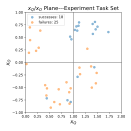
\includegraphics[width=0.6\linewidth]{Figures/xQxO_plane_experiment_set.pdf}
        \caption{(\xQ{}, \xO{}) values of networks sampled for MTurk study.}
        \label{fig:exp_set}
    \end{figure}

    \noindent \paragraph{Participants}
    The total number of participants represented is N=255, with $n=\{63,63,64,65\}$ for conditions 1-4 respectively. The results of two participants were not included because of inability to follow the instructions satisfactorily. Participants were paid a base rate of $\$1.60$ for the Human Intelligence Task (HIT), and were able to get a bonus of up to $\$1.00$ based on their performance. Pilot data indicated that this would be equivalent to approximately \$7-10/hr. In practice the Turkers were quite a bit faster than those in the pilot study, and earned around \$13/hr.
